\documentclass[a4paper]{article}

\usepackage[english]{babel}
\usepackage[utf8]{inputenc}
\usepackage{amsmath}
\usepackage{graphicx}
\usepackage[colorinlistoftodos]{todonotes}
\usepackage{hyperref}


\title{Energy Management Strategies on an Islanded Microgrid with Integrated Renewables and Storage}

\author{Abhilash Kantamneni, Kalin Lee}

\date{\today}

\begin{document}
\maketitle

\begin{abstract}

% Brief Abstract

As installed cost of renewables continues to decrease around the world, providing reliable and affordable energy is starting to become a challenge for grid operators due to the intermittent and non-dispatchable nature of renewable energy sources. This project examines a very simplified process of planning, designing and dispatching generation using the example of a five-bus microgrid system containing distinct resource types. The resources consist of conventional dispatchable generation, non-dispatchable generation from renewable resources, as well as integrated demand response. Economic dispatch of generators was done by DC OPF within generator constraints . The report includes a discussion on the performance of the approach along with its merits and demerits.Historical load and generation data were used as inputs. The microgrid was operated for cost minimization within operating constraints.
\end{abstract}



\section{Introduction}

Over the past decade, the average utility electric rates across the world have continued to increase even while the per capita annual household consumption of electricity has seen a steady decline due to the energy efficiency policies and technologies \cite{simshauser2012energy}. Additionally, a combination of favorable government policy, tax incentives, financing options, public awareness about climate change and emerging markets for renewable energy technology has driven down the cost of renewable system deployment in many parts of of the world. According to a new report\cite{feldman2014photovoltaic} by the US National Renewable Energy Laboratory, in the United States alone the price of solar energy has seen a double digit decline in 2013, with trends expecting to continue to meet the US Department of Energy's SunShot target of making solar energy cost competitive with traditional energy sources by the year 2020 \cite{sunshotus}. Wind power has recently become the fastest growing renewable energy resource and is projected to lead the growth of the renewable power portfolio in the near term\cite{tarroja2012metrics}.

A combination of those two factors has put rooftop solar and wind within the reach of many households in America. As renewable energy innovations see a surge in deployment on rooftops (PV) and farms(Wind), these technologies are increasingly being percevved as a threat to the business model of conventional utilities \cite{graffy2014does}. This disruptive competition from renewable energy sources offers the possibility of fundamentally transforming the electric market structure. In energy markets with increasing proliferation of non-dispatchable and intermittent generation sources, balancing generation and loads in real time is starting to increasingly become a challenge for market operators. 

What is the impact of intermittent renewable energy generation on the electric load demand? How can generation sources be sized, utilized and their dispatch be coordinated to balance load in real time? What are the thresholds for reliable penetration of renewable sources on a grid? How can reliability and operational cost be optimized simultaneously? 

In this paper, such problems are studied in the context of an islanded microgrid with integrated storage and demand response. A complete description of the system and problem statement is provided in Section \ref{Problem Statement}.

 



\section{Literature Survey}

\subsection{Does Disruptive Competition Mean a Death Spiral for Electric Utilities?}

Graffy and Kihm \cite{graffy2014does} discuss the effect of the surge in rooftop solar on the future shape and status of electric utilities, and its implications for industry and society. The authors argue that the characterization of renewable energy technologies as a 'threat' to conventional utility business models reflects the awareness of emerging unconventional risks with the availability of safe, secure and accessible energy.  They propose that \textit{disruptive competition signifies a synergistic wave of innovations occurring in several sectors at once
 — 
technology research and development, policy development, social and cultural preferences, scientific investigation, and business}. 

They argue that the current quasi-public monopolistic model of regulated utilities in America are ill-suited to meet emerging demands on the energy sector when facing such disruptive competition. They propose that the short term tactics employed by certain utilities\cite{marc} in fighting rooftop solar by imposing feed-in tarrifs, and net-metering limits are unsustainable. In fact, such efforts \textit{might perversely increase the risks of a death spiral by ignoring the vulnerabilities of the legacy model and squandering critical assets that are required for successful adaption}. Instead, the authors predict that utilities can successfully compete against this emerging paradigm only by integrating renewables into attractive products and services offerings, with the possibility of a revised price structure.

An illustrative analogy used by the authors is striking: How the music industry as unprepared to adopt to the disruptive innovation of Napster and iTunes, and was forced to adopt. 

In this project, we propose a utility market with no feed-in tarrifs, no fixed costs, and no limitations on net-metering capacity limits. A complete analysis of a 'fair' customer credit for excess generation is beyond the scope of this report. 

\subsection{Optimisation of energy management in commercial buildings with weather forecasting inputs: A review}
Lazos et al.\cite{lazos2014optimisation} discuss numerous methods available in literature, of using statistical or physical algorithms for predicting a building's load and gneneration for optimizing energy management. The paper discusses the strengths, weaknessess, and applications of different algorithms for  predicting building loads using weather forecast over different prediction horizons. 

While weathers forecasts incorporated by ISOs and grid operators into their unit-commitment and economic load dispatch models, for the puposes of this term project, sample load profiles for residential, commercial and industrial buildings at 1-hour granularity for a period of one whole year were obtained from publicly available databases \cite{clain1generating}. 

\subsection{Metrics for evaluating the impacts of intermittent renewable generation on utility load-balancing}
Tarroja et al \cite{tarroja2012metrics} developed metrics to evaluate the impact of intermittent renewable generation on the electric load demand. 

They argue that while wind and solar power offer several benefits to the grid operator like nearly zero fuel, operation and maintainence costs, they also pose a great challenge to grid integration stemming from intermittent generation that is independant of load demand. Reliable sypply of power to customers is managed by balancing load and demand at all instances of time by optimizing parameters such as marginal cost of operation, minimum operating time, maximum power, grid congestion constraints and other constraints. They arguel that \textit{The projected introduction of high penetration levels of wind and solar power into the electric grid mix introduces a degree of uncertainty and variability into the electric power generation component.} 

The authors suggest a typical balancing structute for a grid to meet NERC standards, containing three predominant operational categories:

\textit{Base-load}: Base loaded generators operate for very long time periods and typically encompass large-scale power plants that exhibit high efficiencies, low operating costs and use nuclear or coal fuel.

\textit{Load-following}: Load following generators provide energy to meet daily and hourly variations in the predicted electric load demand above the portion that is met by base-load generators. Their operation is characterized by short ramp times and have typically higher operational and fuel costs and are typically used to meet spinning reserve requirements. 

\textit{Peaker}: Peaking generators provide energy when load-following capacity and flexibility are insufficient to meet the load while maintaining regulation and reserve margins.

The authors argue that \textit{high renewable penetration levels could impose severe challenges for the balance generator fleet and implied costs of installing and operating such a fleet without energy management strategies.}

For the purposes of this paper, a coal based plant is used for baseload generation and a gas fired generator is employed as a peaker-plant for load following.  

\subsection{Generation unit commitment in microgrid with renewable generators and CHP}

Thammasorn\cite{thammasorn2013generation} utilized unit commitment to determine the required battery capacity for a power system. The system consisted of electric loads, heating loads, and variable generation. The unit commitment problem was divided into the power flow calculation and the unit commitment problem. However, it is not clear what, if any, optimization method was employed. The IEEE 14-bus cast study was used for the model. A wind plant was connectd at bus 2, a solar plant at bus 3, CHP plants at buses 5 and 6, a gas engine at bus 8, and battery storage at bus 1. 

This paper will help us in developing generation models for intermittent wind and PV sources along with models for conventional gas generators and energy storage device. The most crucial component of this paper for our project will be with helping determine the appropriate battery capacity.

\subsection{A Unit Commitment Model with Demand Response for the Integration of Renewable Energies}

Ikeda et al.\cite{ikeda2012unit} developed a unit commitment model based on mixed integer linear programming (MILP) in order to analyze “requirements of the forecast output and its error for renewable energies”. The demand response status and the forecasted demand are some of the objective function’s independent variables. The forecasted demand error and forecasted generation error are considered in the constraints.

The model consisted of 12 thermal power plants totaling 188 MW, 30 MW of solar capacity, and 30 MW of wind capacity. The peak demand was about 170 MW. The error (i.e., standard deviation) was specified for cases of 10\%, 20\%, and 30\% of the capacity. The reference case used the thermal power plant and variable generation (VG).

The VG was absorbed by starting the thermal plants serially in merit order. The marginal cost was highest during daytime hours due to high demand, demonstrating a typical price structure. The operation cost was demonstrated to increase with forecast error. A wind down-ramp was analyzed, which requires more thermal plants to be operated, however the effect was small due to the short time period affected. Demand response (with wind) was demonstrated to reduce the number of thermal plants operating.

While the paper focuses on traditional power plants, the approaches in this paper will help us develop the unit commitment model of our microgrid by developing an objective function as a time series of the operational state of the microgrid. The paper will also help us calculate the global constraints like demand response limits and local constraints like generation unit, ramp up/down constraints etc. 

% \subsection{Multi-Agent System (MAS) for short-term generation scheduling of a microgrid}
% Logenthiran et al.\cite{logenthiran2010multi} propose a multi-agent system for generation scheduling of a microgrid, that has individual agents for controlling sources, loads, and storage in a three-level architecture. Individual agents at sources (SC Agent) can model Distributed Energy Resources (DER) and maximize their power production subject to production cost and unit constraints, while agents at the load end help with managing demand response by controlling loads. These agents are controlled by a microgrid management (MGM) agent, in either centralized or decentralized manner, and the paper allows for some discussion on the relative merits of either approach, which will aid us in developing a control architecture for our project's case study.

% While the paper uses an additional layer of control, the distribution management system (DMS) agents to control individual MGM agents, our analysis will be restricted to a two-level architecture at the MGM level, since our project is only concerned with the optimal operation of a single microgrid. However, the discussion in the paper on the role of the DMS agents will help us chart future extentions of our project. 

% This paper will also help us develop a model for unit commitment of each generation and subsequent bidding strategies of the generation agents and the load agents, through the formulation of full-load average production cost (FLAC). The discussion on strategies for bidding under incresing/decreasing generation/load conditions, and their subsequent interaction with the storage agent is valuable to our project's case study.

\subsection{Modelling high level system design and unit commitment for a microgrid}

Hawkes and Leach\cite{hawkes2009modelling} use a linear programming model to minimize the equivalent annual cost (EAC) of meeting a given energy demand. They calculate the total EAC including the annual cost of electricity, fuel and maintanence and the annualized cost of the generation units required an subtracts any revenue gained from exporting electiricy to the grid. In our test case however, no revenue is offered by our utility for net excess export, but the grid can be used as a load bank for demand response, for up to 300 kW.

We intend to follow the same constraints that were modeled in this paper including the inability of a unit to exceed its rated capacity, ramp limits for each generator, charge/discharge rate limits for each storage unit, onsite load must be met exactly, since the microgrid does not expect to be operated in the islanding mode, heat demand must be met or exceeded, and electrical or thermal energy stored in one season may not be transferred to another season. 

While the paper considered many components of the microgrid, for the purposes of our paper we will employ up to three natural gas generators, 20 kW of solar PV capacity, and model a 50 kW wind turbine. While the paper uses boilers as a storage for thermal energy, we intend to use a 80 kW, 160 kWh battery. The paper also models the performance of microgrid in the islanded mode, which provides additional energy security in the event of grid failure. 

We intend to use this paper to provide insight and direction into calculating the lifecyle cost of energy produced by our assets in the microgrid, and into calculating the payback period for investing in such a resource using Monte Carlo simulations for different conditions outlined in the paper (e.g., future increase in utility rates or natural gas prices). The paper has an interesting discussion on reducing the aggregate cost of all microgrid participants versus optimizing for individual partnerships. Concepts raised in this discussion will help our project with resolving any Prisoner's Dilemma/Game Theory situation of resolving tension between cooperative partnerships and self interest motivations for microgrid participants in our project's case study.

 
\section{Problem Statement}
\label{Problem Statement}

What is the optimal strategy for managing a grid with integrated renewable generation? 

When designing a new generation facilities, major parameter decisions to be made include choices of generation fuel, type of generation system, plant rating, siting and a number of technical, economic and enviroinmental factors. Inspired by a step-by-step process developed by Shalaan \cite{shaalan2003generation} we aim to design a grid with adequate mix of generation sources to reliably and affordabily meet the energy needs of a small hypothetical town called 'Huskyville'. 

% % FIG1
\begin{figure}[h!]
\centering
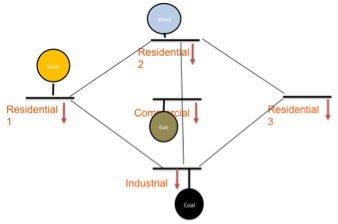
\includegraphics[width=0.9\textwidth]{FIG1a.png}
\caption{\label{fig:FIG1a}The five-bus microgrid system indicating generation resource by bus.}
\end{figure}

\subsection{Identify loads and generate load profiles} 

A microgrid was modeled as a simple five-bus system with loads and distinct resources on each bus, depicted in figure~\ref{fig:FIG1a}. Three bus loads represent residential loads (Bus 1-3), one bus load represents a commercial load (Bus 4), and the fifth bus load represents an industrial load (Bus 5). The characteristic loads at each of the buses is given in Table \ref{tab:BusLoads}. The load profile of an average day is given in Figure \ref{fig:LoadProfile.png} A complete load profile of each individual bus for each hour of one year is given in Appendix A. 

Load profiles were obtained from publicly available data from CAISO, NE-ISO, and MISO. Generation profiles for solar and wind, displayed in Figure, are from publicly available data from NSRDB and ERCOT.


% % FIG1 Load Profiles
\begin{figure}[h!]
\centering
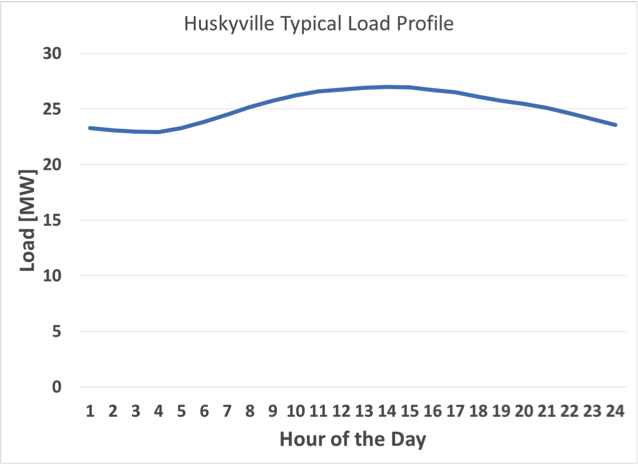
\includegraphics[width=0.9\textwidth, height=0.15 \textheight]{LoadProfile.png}
\caption{\label{fig:LoadProfiles} The load profile of the microgrid on an average day. The peak load is ~27MW}
\end{figure}



\begin{table}
\label{tab:BusLoads}
\centering
\resizebox{\textwidth}{!}{%
\begin{tabular}{|c|c|c|c|c|}
\hline
\textbf{Load Type} & \textbf{Bus Number} & \textbf{\begin{tabular}[c]{@{}c@{}}Average Peak Load\\ {[}kW{]}\end{tabular}} & \textbf{Number of Units} & \textbf{\begin{tabular}[c]{@{}c@{}}Bus Peak Load\\ {[}MW{]}\end{tabular}} \\
\hline \\
\textit{Residence 1} & 1 & 3.04 & 700 & 2.13 \\
\textit{Residence 2} & 2 & 4.08 & 700 & 2.85 \\
\textit{Residence 3} & 3 & 1.61 & 700 & 1.13 \\
\textit{Commercial} & 4 & 35.10 & 100 & 3.51 \\
\textit{Industrial} & 5 & 8820.00 & 2 & 17.6 \\ \hline
\textbf{Total} & - & - & - & \textbf{27.0} \\ \hline
\end{tabular}}
\caption{Typical average daily peak loads of each individual unit. A complete load profile for each hour of the year is available in Appendix A}
\end{table}



\subsection{Identify sources and eliminate alternatives}
  Out of the entire possible fuel mix available to a location in the United States of America Figure \ref{fig:Sources}, nuclear was eliminated due to system unavailability (too big), hydropower and geothermal were eliminated due to fuel unavailability at location, biomass was eliminated due to funtional unavailablity (high capital costs). 
  
  
  % FIG1 Load Profiles
\begin{figure}[h]
\centering
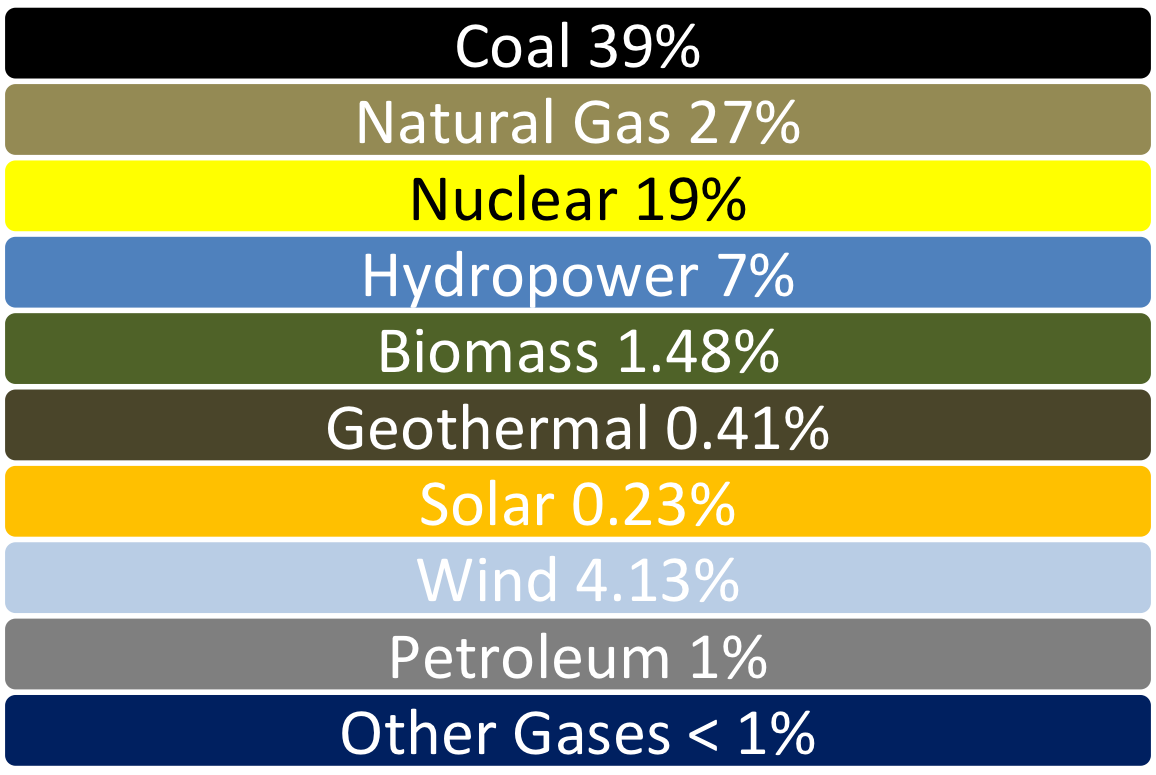
\includegraphics[width=0.9\textwidth]{Sources.png}
\caption{\label{fig:Sources} US electricity by fuel source 2013. Data from Energy Information Administration www.eia.gov}
\end{figure}
  
Of the remaining sources, a coal based plant is used for baseload generation and a natural gas fired plant is used for load following/peaking generation. The base load plants have low fuel costs, but minimal ramping capability, and the peaking plants have higher fuel costs and more flexibility. Renewables areintegrated into this grid by allowing residential customers to net-meter solar and wind to their homes. For demostration purposes, it is assumed that area Residence 1 (Bus 1) only installs solar and Bus 2 residents only install wind.  

Furthermore, it is assumed that each house only installs a renewable energy system that can generate enough electricity to power the energy needs of that house over one year. Framed differently, the cumulative energy generated at each bus 1 and 2 over one year is equal to the net energy consumed at that respective bus over one calendar year. 
\subsection{Determine Generation Capacity}

Baseload generation is sized to meet the minimum electric load demand over the system. Peaker plants are sized to meet the sudden spikes in demand within a day or hour cycle. Based on the cumulative load profiles on the Huskyville microgrid for the whole year (Figure \ref{YearlyLoadProfiles} ), it is clear to see that the maximium capacity of a basload generator is 20MW. This is additionally augmented with a natural gas peaker plant. 

At every single hour of the year, the capacity of renewable energy generation is determined as a ratio of penetration from maximum resource potential at given location. This is explained in detail in section \ref{case}

\begin{figure}[h!]
\centering
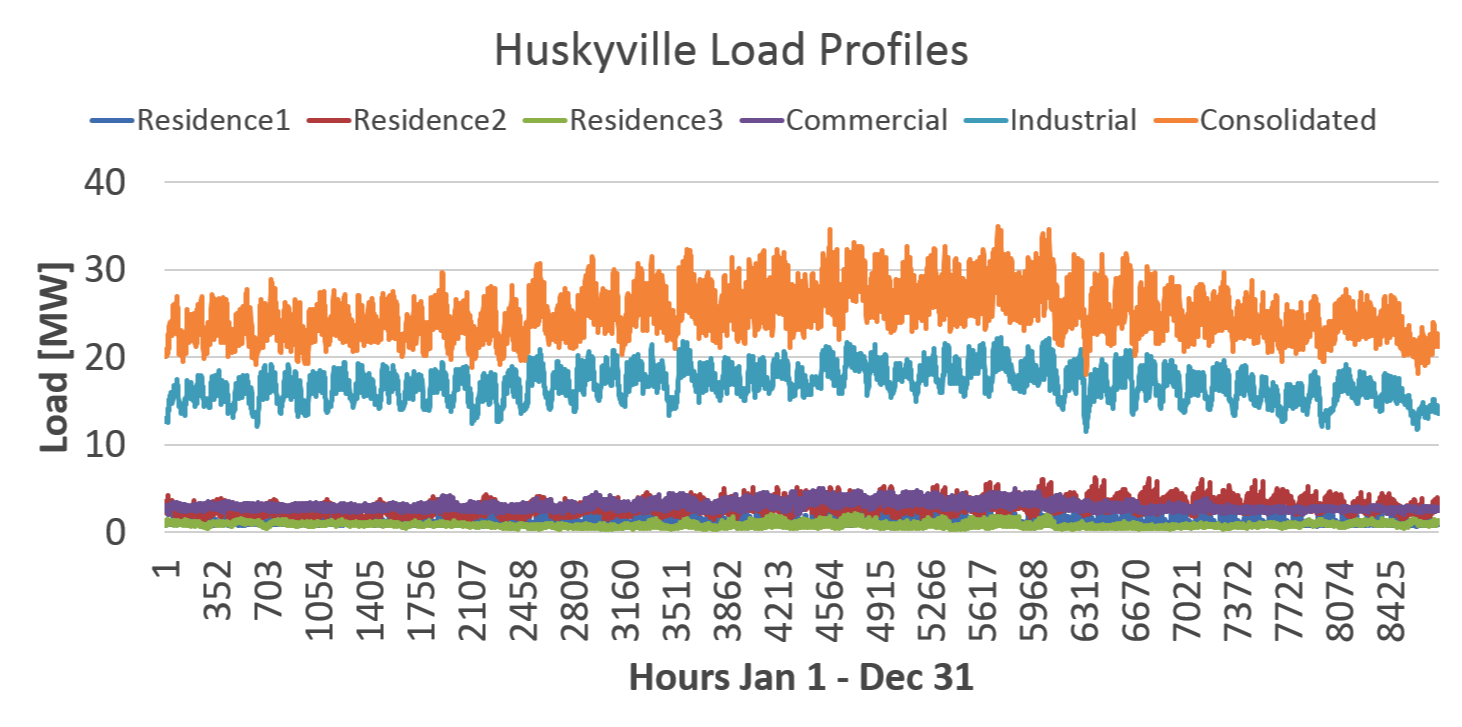
\includegraphics[width=0.9\textwidth]{YearlyLoadProfile.png}
\caption{\label{fig:YearlyLoadProfiles} The load profile of the microgrid over one year. A complete load profile for each hour of the year is available in Appendix A}
\end{figure}

Figure \ref{fig:FIG3} shows the renewable resource profile for every single hour of one year.  

% FIG3
\begin{figure}[h!]
\centering
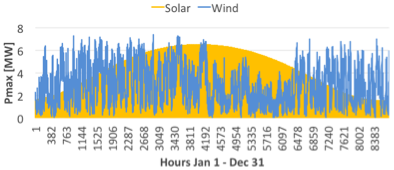
\includegraphics[width=0.9\textwidth]{FIG3.png}
\caption{\label{fig:FIG3}Solar and wind generation profile.}
\end{figure}

\subsection{Model Cost Curves and Determine Operation Costs}
 
% The most fundamental constraint of a power system is the balance of generation and load. Generation units must be committed and dispatched using algorithms that optimize the cost. Resource characteristics can be considered as well, such as dispatchability, variability, and commitment cost.

% A microgrid may include renewable resources, such as wind and solar generation, along with conventional generation. Renewable resources reduce operational fuel costs. Base load and peaking plants must still be operated. 

% Other solutions to resource integration are demand response, curtailment of non-dispatchable generation, and energy storage, which can support minimizing system cost. However these methods have their own constraints and dispatch strategy can significantly affect the system effect.

Costs of operating each of these generation facilities can be adequately appromixated to a piecewize linear cost function. This function can encapsulate within it both fuel I/O curves and the fuel cost curves \ref{fig:Costs}.

\begin{figure}[h!]
\centering
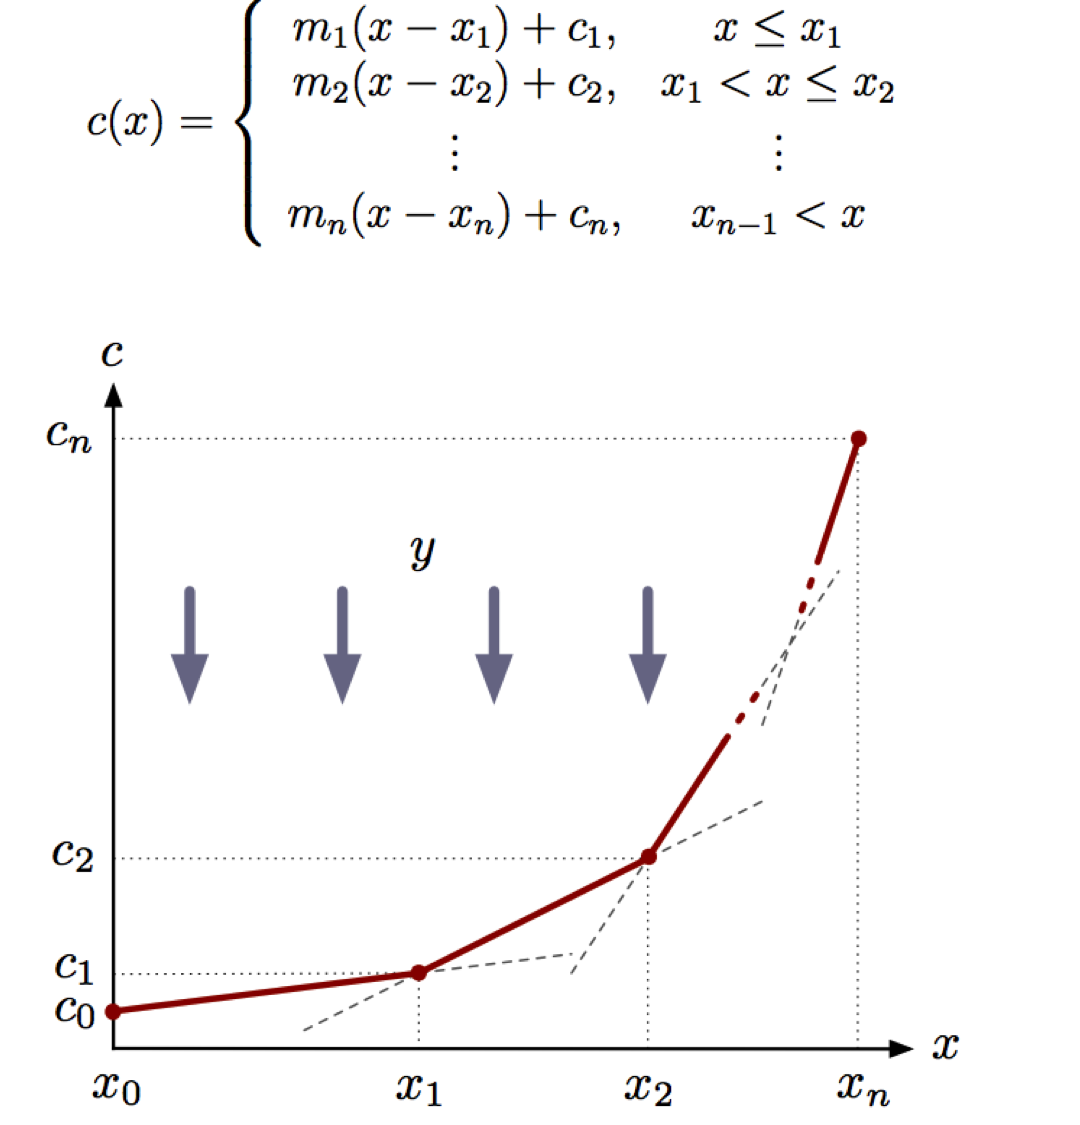
\includegraphics[width=0.6\textwidth]{Costs.png}
\caption{\label{fig:Costs}Piecewize linera cost function as a model for generator costs.}
\end{figure}

Base load coal generator can operate for very long time periods and has low operating costs, but is very expensive to turn up or turn down. Load following natural gas generators has typically higher operational and fuel costs , but low ramp up and ramp down costs, and can be turned on and turned off inexpensively. While the installed cost of renewable systems might be high, they have practically no operational cost so their fuel costs are assumed to be zero. 

A summary generator characteristics and cost function constants are shown in figure~\ref{fig:FIG2}. 


% FIG2
\begin{figure}[h!]
\centering
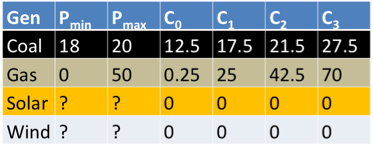
\includegraphics[width=0.9\textwidth, height=0.25\textheight]{FIG2.png}
\caption{\label{fig:FIG2}Generator unit limits and cost function parameters.}
\end{figure}

The economical operation of this microgrid susbequently boils down to an economic load dispatch problem, which is explained in great detail in the subsequent section.

\section{Theory}
The challenge a market operator faces lies in using a combination of available generation sources to meet changing load demand reliably and affordably. This is essentially a high-level optimization problem of miniminizing cost while making sure all the linear and non linear system constraints are not violated. This problem can be split into as two complementary components:


\subsection{Economic Load Dispatch}

The economic dispatch of committed generators requires an optimization method such as dynamic programming, duality methods, and genetic algorithms.

A duality method, such a Lagrangian Relaxation, relaxes the problem by ignoring alternately the constraints and the cost function. This creates two simplified problems, a primal (cost minimization) problem and a dual (constraint-penalized) function. The method iteratively solves the primal and then the dual problem. However, the method can take a long time, can result in a close, but imprecise, solution,and is d ifficult to incorporate a transmission constraint.

The optimal power flow (OPF) method can solve economic dispatch with a transmission constraint. The problem takes the form min\_x(f(x)), subject to g(x) = 0, h(x) <= 0, and xmin <= x <= xmax. x represents voltage angle (Theta), voltage magnitude (Vm), real power, and reactive power. However, the problem can be simplified by assuming constant voltage angles and magnitudes. This limits polynomial cost functions to second order, simplifying the (AC) OPF problem to a quadratic problem with linear constraints. This simplified OPF is called DC OPF because it is of the same mathematical form (i.e., linear) as Ohm’s Law.

\subsection{Unit Commitment}

Unit commitment is a similar type problem as economic load dispatch, requiring an optimization routine. However, rather than providing the optimal dispatch, the problem uses the dispatch to determine the optimal commitment of each generator unit.For a simple microgrid, with only one generator of each resource type, unit commitment is not necessary. Non-dispatchable generation will be always on. Base load generation must be on at low to moderate renewable penetration to maintain the system, while peaking generation will remain on for the marginal load.



\section{Simulation}
\label{case}

Our project used the following assumptions to calculate the minimal operating cost under different renewable energy deployment scenarios: Generation capacity limits and costs as indicated in Figure , no spinning reserve requirements, transmission losses are ignored and no emission constraints. 


The model was simulated at several renewable resource penetration levels. The hypothetical cases 10\%, 50\%, and 100\% of residents install a net metered reenwable system. 

The OPF problem was solved using MATPOWER\cite{zimmerman2011matpower}, an open-source Matlab-based power system simulation software. For every single hour of one year, MATPOWER's OPF solver was run to identify the optimal generation dispatch under each of the test cases. 

\subsection{Case 1: 10\% residential renewable penetration}

In this case study, 10\% of all residents in Bus 1 and Bus 2 install a net-metered renewable system. In other words, at each hour of the whole year, the available capacity of renewable energy generation is 10\% of maximum available potential as described in Figure ~ref{fig:FIG3}. 

A sample case of 10\% renewable resource penetration is seen in figure~\ref{fig:FIG4}. The marginal cost is \$164.01/MWh. The energy mix is 1.1\% solar, 1.5\% wind, 21.0\% natural gas, and 76.4\% coal. The renewable resource generation had negligible impact on dispatch, but simply reduced system slightly cost by reducing fuel cost.

% FIG4
\begin{figure}[h!]
\centering
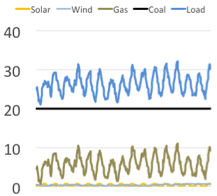
\includegraphics[width=0.9\textwidth , height=0.25\textheight]{FIG4.png}
\caption{\label{fig:FIG4}10\% residential renewable penetration for first 12 days of the year. Charts for the full year are available in the appendix}
\end{figure}

\subsection{Case 2: 50\% residential renewable penetration}

In this case study, 50\% of all residents in Bus 1 and Bus 2 install a net-metered renewable system. In other words, at each hour of the whole year, the available capacity of renewable energy generation is 50\% of maximum available potential as described in Figure ~ref{fig:FIG3}. 

The case of 50\% renewable resource penetration is seen in figure~\ref{fig:FIG5}. For the full year, the marginal cost of is \$111.01/MWh. The energy mix is 5.2\% solar, 6.8\% wind, 11.7\% natural gas, and 76.3\% coal. The renewable resource generation reduced expensive natural gas fuel cost significantly, but only impacted base load coal dispatch slightly.

% FIG5
\begin{figure}[h!]
\centering
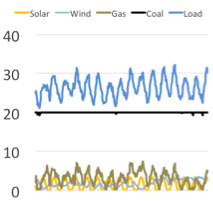
\includegraphics[width=0.9\textwidth , height=0.25\textheight]{FIG5.png}
\caption{\label{fig:FIG5}50\% residential renewable penetration.}
\end{figure}

\subsection{Case 3: 100\% residential renewable penetration for first 12 days of the year. Charts for the full year are available in the appendix}

In this case study, all residents in Bus 1 and Bus 2 install a net-metered renewable system. In other words, at each hour of the whole year, the available capacity of renewable energy generation is simply maximum available potential as described in Figure ~ref{fig:FIG3}.

A sample case of 100\% renewable resource penetration is seen in figure~\ref{fig:FIG6}. For the full year, the marginal cost is \$126.37/MWh. The energy mix is 10.7\% solar, 13.6\% wind, 17.5\% natural gas, and 58.2\% coal.

Since the operation cost of renewables is essentially free, the renewable resources are dispatched first. AS a result, on occasion there isn't enough load for the coal plant to service. In other words, the available load is lesser than $P_{min}$ of the coal based plant. As a result, the coal plant is decomissioned so as to not violate the $P_{min}$ constraint. This means that the expensive gas fired peaker plant provides a makority of load support.  

So even though the cost of energy generated by renewables is cheap, the over all marginal cost of generation with 100\% residential renewables is higher than Case 2 with only 50\% penetration.  

% FIG6
\begin{figure}
\centering
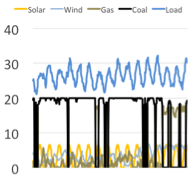
\includegraphics[width=0.9\textwidth , height=0.25\textheight]{FIG6.png}
\caption{\label{fig:FIG6}100\% residential renewable penetration for first 12 days of the year. Charts for the full year are available in the appendix}
\end{figure}

\section{Energy Management Strategies}
We propose two smart strategies for energy management to dispatch generation in the event of such high penetration of renewables
\subsection{Generation Curtailment}
A simple solution is to curtail generation from renewable sources at times when the alternative would be decomissioning the baseload generation. In the real world, this is achieved through scheduling unit commitment based on forecasts of load and renewable generation. Since renewables do not have a ramp up or ramp down costs, energy from renewables can simply be taken 'off-line'. 

The inclusion of curtailment in the dispatch can mitigate this problem and maintain the base load generation above a minimum threshold, depicted in figure~\ref{fig:FIG7}. The marginal cost is \$86.02/MWh. The energy mix is 8.1\% solar, 9.5\% wind, 7.5\% natural gas, and 74.9\% coal. This reduces the energy contribution of renewable resources to an amount between the 50\% and 100\% penetration. As seen in figure~\ref{fig:FIG7}, baseload generation us unaffected, but gas fired generation is ramped up. 

Renewable generation often serves social, political, and environmental purposes as well so this reduction must be carefully considered in any regulatory process. Frequent curtailment can distort the Levelized Cost of Energy and economic Return on Investment for third-party renewable energy developers. Within the U.S. production tax credits, which are only incurred for actual energy produced, would also have to be considered or compensated. Many states in America also have strictly enforced Renewable Porfolio Standards for regulated utilities, where utilities are mandated to meet 10\% of their generation portfolio through renewable energy sources which places an additional constraint against overuse of generation curtailing as a energy management strategy. 

%FIG7
\begin{figure}
\centering
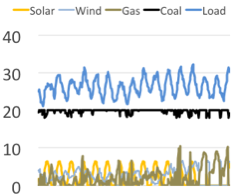
\includegraphics[width=0.9\textwidth , height=0.25\textheight]{FIG7.png}
\caption{\label{fig:FIG7}100\% residential renewable penetration with generation curtailment. Charts for the full year are available in the appendix}
\end{figure}

\subsection{Integrated Storage}

The case of 100\% renewable resource penetration with storage is a complex implementation due to complicated control options. There are many control strategies for storage, which can impact dispatch and system in different ways. For the purposes of this project, storage was implemented in the form of EV-to-Grid technology. It is assumed that all residences in Bus 3 have an Electric vehicle that is connected to the grid at almost all times. The control scheme for charging and discharging EV is implemented as follows:

When the load demand is less and there is a danger of baseload generation being decomissioned, load can be dispatched in the form of demand response. IN other words, EV vehicles connected to the grid begin charging. During periods of low demand, EVs appear as load on the grid. During other times, EVs appear as generators. We implemented a simple control where EVs retain a portion of their charge and only discharge a maximum of 60\% back into the grid. The charge and discharge cycles are assumed to be completely efficient.

%FIG7
\begin{figure}
\centering
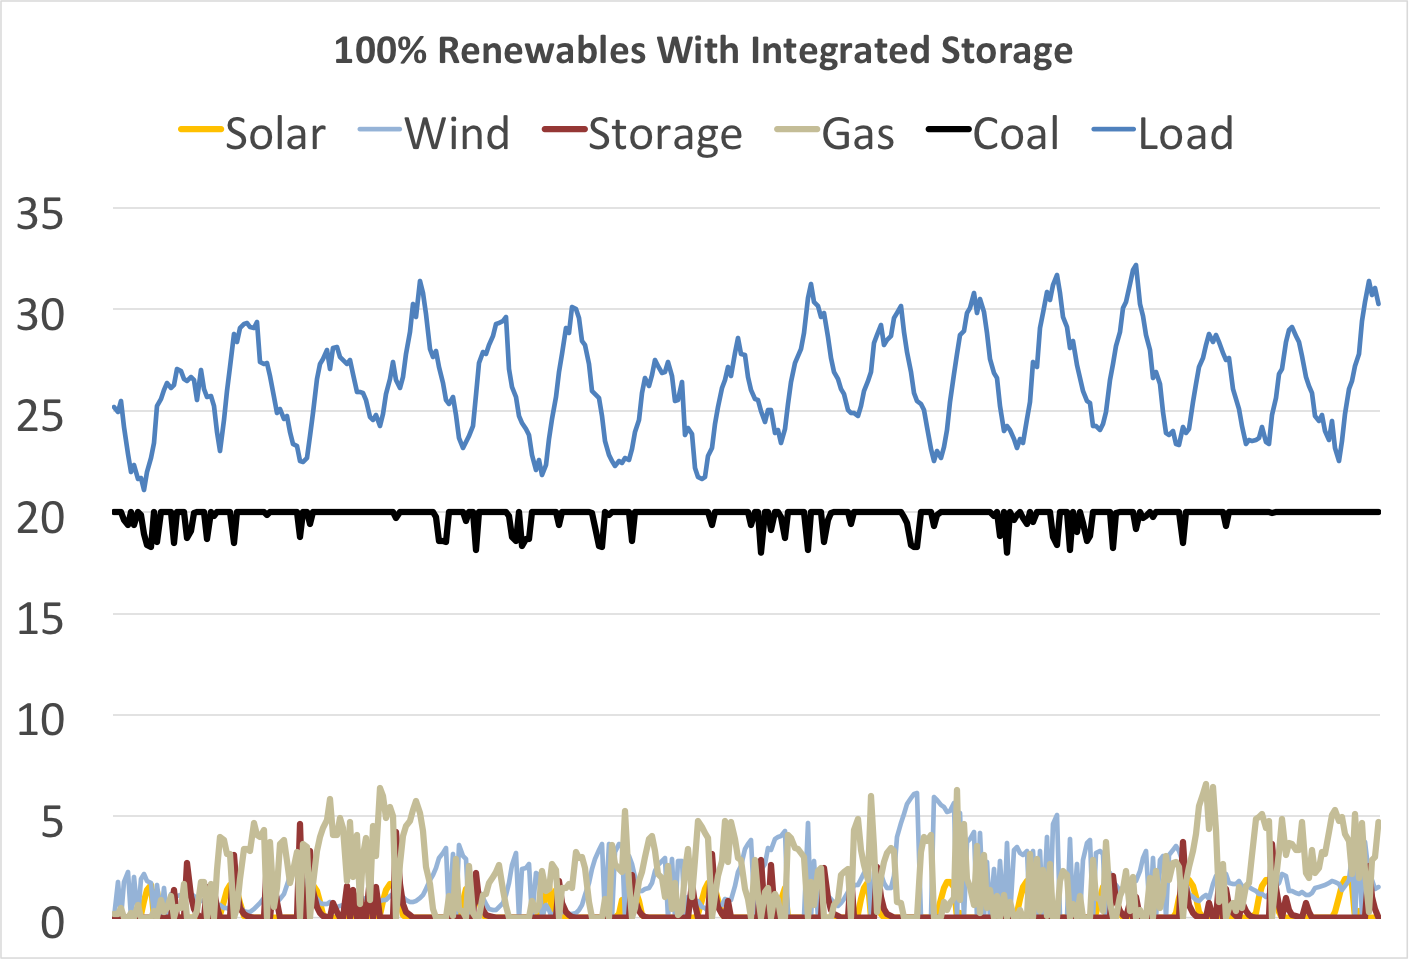
\includegraphics[width=0.9\textwidth , height=0.25\textheight]{Storage.png}
\caption{\label{fig:FIG7}100\% residential renewable penetration with integrated storage. Charts for the full year are available in the appendix}
\end{figure}

The marginal cost is \$101.89/MWh. The energy mix is 6.4\% solar, 7.5\% wind, 3.5\% from storage, 13.5\% natural gas, and 74.9\% coal.  



\section{Discussion}

The simulation of economic dispatch with dc optimal power flow shows the benefits of renewable resource generation from zero fuel cost, but also some of the dispatch problems created from non-dispatchable, variable generation, as well as some solutions.The work indicates that a minimal penetration (e.g., 10\%) of renewable generation has little impact on the system, except for reduced operating costs. Even a significant (e.g., 50\%) penetration has little negative effect, but greatly reduces operating costs. Real-world examples, such as Ireland, with significant wind, and Germany, with significant wind and solar, corroborate this result.

A very large penetration (e.g., 100\%) of renewable resources, of greater magnitude than existing peaking and non-base load generation, will impact dispatch. The decommitment of base load generation will lead to significant peaking generation increasing fuel cost.

Integration of renewables can be achieved using smart energy management strategies.   



\section{Future Work}

For high-penetration cases the impact of base load generation cycling is unknown. The case, without curtailment or other mitigating solutions, is not positive, and any cycling cost may make the case worse. Long-term analysis should determine any lifetime impact on the base load generation from cycling. The impact could be translated to a shadow price, which could then be used in short-term studies.

Energy storage requires extensive future work due to the many control strategies available. Storage can also be used for more localized purposes, such as infrastructure deferral and mitigation of transmission constraints. Control strategies should consider the capability to offer multiple services.

The energy management strategies proposed are naive and for illustrative purposes only. In real world operation, load and generation forecast data are obtained using either AI or stochastic means and are prone to error and fuzziness. The work in this paper can be extended for a real world case by removing some of the assumptions with respect to line losses, charge efficiency and other assumptions.

The test microgrid can also be interconnected with neighboring areas to export and import energy. As long as nearby areas have non-coincident peak demand and supply, grid interconnection provides a lot of reliability benefits. 

\section{Contributions}

Abhilash Kantamneni

\begin{itemize}
\item Development of outline.
\item Literature Review
\item Development of model.
\item Integration of model with Matpower.
\item Presentation.
\item Development of final report.
\end{itemize}

Kalin Lee

\begin{itemize}
\item Development of outline.
\item Development of alternative models (Lagrangian Relaxation), not used in final simulation due to lack of transmission constraint.
\item Development of storage modeling.
\item Development of draft report.
\end{itemize}

\section{Appendix}

In the interest of being concise, data and charts have been uploaded to github: \url{'https://github.com/akantamn/EE5230-Project/blob/master/Presentation/Solutions.xlsx'}

\bibliographystyle{IEEEtran}
\bibliography{Microgrid.bib}

\end{document}